% Marco teórico - Microfísica
%\chapter{Microfísica: Ecuaciones de Estado}
%\thispagestyle{fancy}

% Introducción similar al capítulo sobre macrofísica. Aquí queremos mostrar brevemente la motivación de el estudio de ecuaciones de estado para entender la física de la materia en entornos tan densos y de tan alta energía.

%\section{Ecuaciones de Estado y Ejemplos}

%Definir las ecuaciones de estado (en este caso barótropas) y mostrar brevemente modelos y gráficas de modelos más simples: gas degenerado de neutrones, protones y electrones libres

%\section{Teoría Relativista de Campo Medio}

% Introducir la RMFT y mostrar las ventajas de una teoría relativista efectiva de campos mesónicos que se toman como uniformes mediante su valor medio en el estado base, frente a otros métodos como QCD y los Scrhodinger-based. Hablar sobre las simetrías y sus cantidades conservadas para explicar como se obtiene la expresión para la densidad de energía y de presión en una teoría de este estilo, construida sobre un lagrangeano.

%\section{Modelo del Estudio}

% Introducir el lagrangiano para un modelo que contenga neutrones, protones, electrones (campos esponoriales); un mesón escalar neutro sigma con autointeracciones de hasta 4to orden acoplado a la densidad escalar de nucleones, un mesón vectorial neutro omega acoplado a la corriente vectorial de nucleones y un mesón vectorial isovectorial neutro rho acoplado a la corriente de isospín de nucleones. Luego hallar las ecuaciones de movimiento para los campos, para finalmente llegar a la expresión de densidad de energía y presión. Hablar sobre los parámetros libres de este modelo.

%\subsection{Materia en Saturación Nuclear}

% Definir, explicar (importancia) y mostrar las mediciones de densidad de saturación, energía de enlace por nucleón, modulo de compresión, coeficiente de energía de simetría y pendiente del coeficiente de energía de simetría. Tomar las mismas mediciones de la propuesta.

\thispagestyle{fancy}
\chapter{Microfísica: Ecuaciones de Estado}

La descripción microscópica de la materia en entornos extremos de densidad es un problema de gran complejidad en la física moderna. En estas condiciones, con densidades que exceden significativamente la densidad nuclear de saturación, la materia exhibe comportamientos que requieren marcos teóricos que incorporen efectos relativistas y de muchos cuerpos. La ecuación de estado que gobierna esta materia establece la conexión directa entre la física microscópica de las interacciones nucleares y las propiedades macroscópicas observables de las estrellas de neutrones \cite{oppenheimerMassiveNeutronCores1939}.

La teoría relativista de campo medio surge como una herramienta particularmente adecuada para abordar este régimen, brindando un tratamiento consistente que respeta la causalidad mientras incorpora las interacciones nucleares fuertes \cite{glendenningCompactStarsNuclear2000}. Este formalismo permite extrapolar desde las propiedades conocidas de materia nuclear simétrica hacia las condiciones asimétricas y de alta densidad relevantes para objetos compactos.

\section{Ecuaciones de Estado y Ejemplos}

Una ecuación de estado define la relación termodinámica entre las variables que caracterizan el estado de equilibrio de un sistema físico. Para materia estelar a temperatura cero, consideramos ecuaciones de estado barotrópicas que relacionan la presión $P$ con la densidad de energía $\rho$ mediante (\ref{eq:ecuacion_estado}). Esta relación contiene toda la información termodinámica necesaria para determinar la estructura de equilibrio hidrostático de estrellas de neutrones a través de las ecuaciones de Tolman-Oppenheimer-Volkoff (\sistemaTOV). La aproximación barotrópica es válida cuando los tiempos y escalas característicos de los procesos térmicos son despreciables comparados con las escalas hidrodinámicas y gravitacionales que determinan la estructura estelar. Se desprecia la temperatura debido a que la energía térmica y sus efectos son varios órdenes de magnitud inferiores a las energías internas de la materia en estrellas de neutrones \cite{shapiroBlackHolesWhite2008}.

\subsection{Ejemplo: Ecuación Politrópica}

La ecuación de estado politrópica es uno de los modelos más sencillos para describir materia estelar, estableciendo una relación de ley de potencias entre la presión y la densidad de masa:

\begin{equation}
	P = K \rho^{\gamma},
	\label{eq:eos_politropica}
\end{equation}

donde $K$ es una constante politrópica y $\gamma$ es el índice adiabático. Esta forma funcional, aunque fenomenológica, captura comportamientos asintóticos importantes de sistemas físicos más complejos y brinda soluciones analíticas o semi-analíticas para las ecuaciones de estructura estelar. El índice politrópico $n = 1/(\gamma - 1)$ determina las características de compresibilidad del material: valores bajos de $n$ corresponden a materia incompresible, mientras que valores altos describen sistemas altamente compresibles. Para materia ultra-relativista, $\gamma = 4/3$ ($n = 3$), mientras que para materia no-relativista degenerada, $\gamma = 5/3$ ($n = 3/2$) \cite{chandrasekharIntroductionStudyStellar1970}.

\subsection{Ejemplo: Gas Ideal Degenerado}
\label{sec:gasnpe}

Los modelos más realistas consideran gases degenerados de fermiones. Para materia nuclear compuesta por neutrones, protones y electrones, la ecuación de estado completa debe incluir las contribuciones de todas las especies presentes \cite{shapiroBlackHolesWhite2008}:

\begin{align}
	\rho_{\text{total}} &= \rho_n + \rho_p + \rho_e, \label{eq:densidad_total} \\
	P_{\text{total}} &= P_n + P_p + P_e, \label{eq:presion_total}
\end{align}

donde cada componente fermionica contribuye según:

\begin{align}
	\rho_i &= \frac{g_i}{8\pi^2} \int_0^{p_{Fi}} p^2\sqrt{p^2 + m_i^2} \, dp, \label{eq:densidad_fermi_general} \\
	P_i &= \frac{g_i}{24\pi^2} \int_0^{p_{Fi}} \frac{p^4}{\sqrt{p^2 + m_i^2}} \, dp, \label{eq:presion_fermi_general}
\end{align}

con masas $m_n = 939.6$ MeV, $m_p = 938.3$ MeV, $m_e = 0.511$ MeV y degeneraciones estadísticas (de espín) $g_i = 2$ para todas las especies. Los momentos de Fermi $p_{Fi}$ están determinados por las densidades de número mediante $n_i = \frac{g_i p_{Fi}^3}{6\pi^2}$, de modo que se tienen tres cantidades independientes: las densidades de número de las diferentes especies. Para resolver el sistema, se imponen restricciones adicionales sobre la composición de la materia garantizando el equilibrio termodinámico: la neutralidad de carga eléctrica requiere $n_p = n_e$, mientras que el equilibrio beta débil $n \rightleftharpoons p + e^- + \bar{\nu}_e$ establece la condición $\mu_n = \mu_p + \mu_e$ entre los potenciales químicos, asumiendo que los neutrinos escapan del sistema sin alterar su energía. Estas restricciones permiten expresar todas las densidades en función de un parámetro libre como el momento de Fermi del electrón $p_{Fe}$, lo que reduce el sistema a una parametrización unidimensional.

\begin{figure}[h]
	\centering
	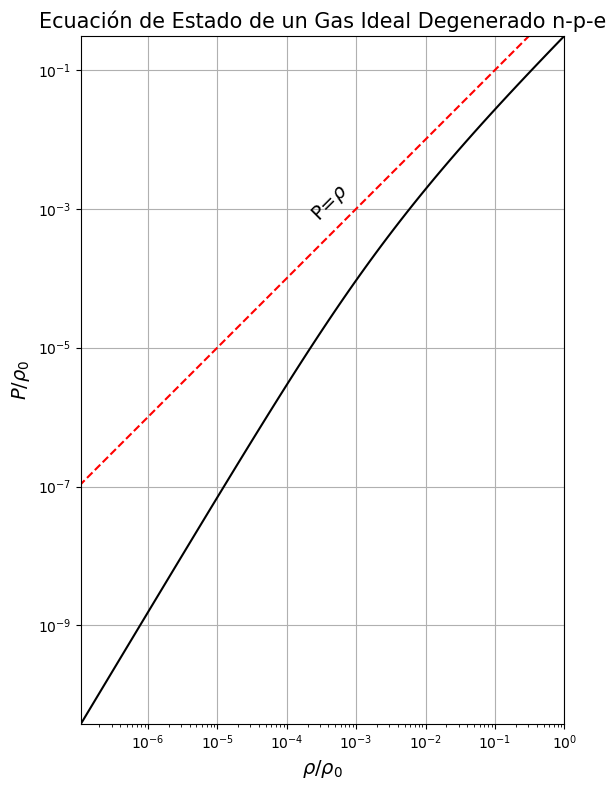
\includegraphics[width=0.55\linewidth]{Figuras/gas_npe}
	\caption[Ecuación de estado de gas ideal degenerado]{Ecuación de estado normalizada de un gas ideal degenerado de neutrones, protones y electrones. La ecuación de estado es causal ($c_s^2 = dP/d\rho < 1$).}
	\label{fig:eosnpe}
\end{figure}

Las integrales (\ref{eq:densidad_fermi_general}) y (\ref{eq:presion_fermi_general}) son analíticas, de modo que la ecuación de estado queda determinada por las expresiones $\rho(n_e)$ y $P(n_e)$ interpoladas sobre un rango de densidades relevante para estrellas de neutrones. El resultado de esta ecuación de estado se muestra en la figura \ref{fig:eosnpe}. Luego, empleando las ecuaciones TOV (\sistemaTOV) obtenemos las masas y radios de estrellas construidas con este material, como se muestra en la figura \ref{fig:mrnpe}. Este modelo sencillo predice una masa máxima de apenas 0.7$\masasol$, muy inferior a las masas que se han observado de estrellas de neutrones (listadas en la sección \ref{sec:obsNS}), motivando la búsqueda de modelos más realistas que logren replicar las observaciones.

\begin{figure}
	\centering
	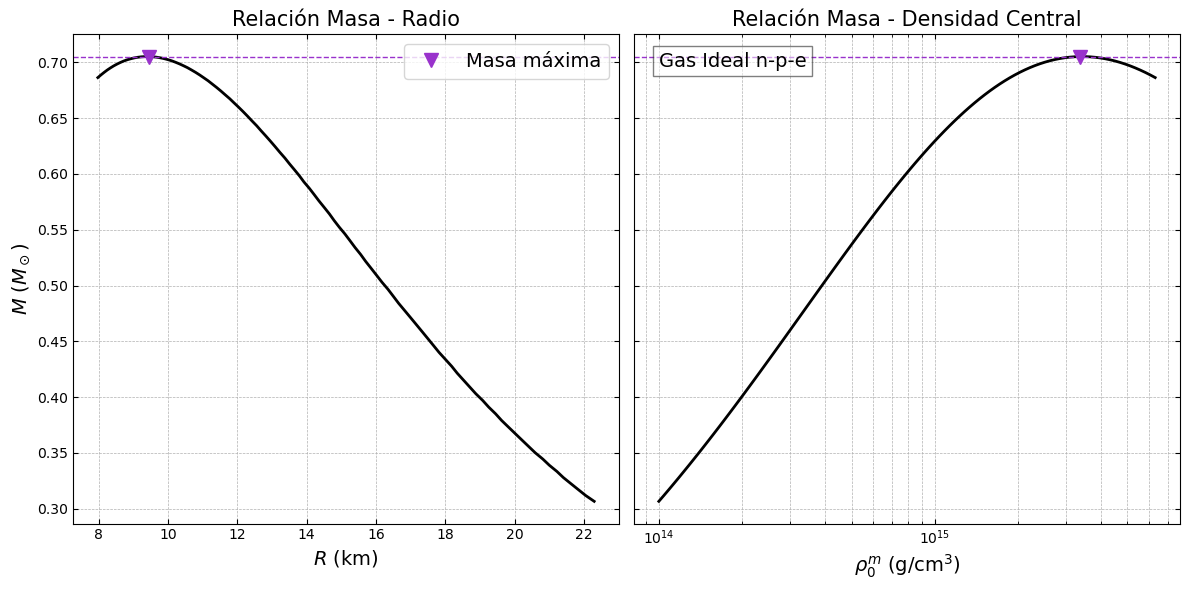
\includegraphics[width=0.9\linewidth]{Figuras/gas_npe_MR}
	\caption[Relaciones masa-radio de gas ideal degenerado]{Relaciones de masa - radio y masa - densidad central de masa de estrellas de neutrones constituidas por un gas ideal de neutrones, protones y electrones libres.}
	\label{fig:mrnpe}
\end{figure}



\section{Teoría Relativista de Campo Medio}
\label{sec:rmft}

La teoría relativista de campo medio es un marco teórico que describe las interacciones nucleares mediante el intercambio de mesones efectivos, extendiendo el modelo de gas degenerado (discutido en \ref{sec:gasnpe}) e incorporando naturalmente las características relativistas en condiciones de alta densidad. Formulada por Walecka en 1974 \cite{waleckaTheoryHighlyCondensed1974}, esta aproximación ofrece ventajas significativas respecto a enfoques no-relativistas basados en potenciales fenomenológicos, particularmente en su construcción covariante, su capacidad para reproducir simultáneamente las propiedades de saturación nuclear, el comportamiento asintótico a alta densidad, y la consistencia causal relativista. Adicionalmente, al ser una teoría efectiva, requiere de un menor esfuerzo computacional respecto a teorías más fundamentales como QCD.

El formalismo se construye a partir de un lagrangiano que describe nucleones interactuando a través de campos mesónicos. Los campos fermiónicos representan los grados de libertad nucleónicos y leptónicos, mientras que los campos bosónicos representan mesones que median las interacciones fuertes. La aproximación de campo medio consiste en reemplazar los operadores de campo mesónicos por sus valores esperados en el estado base degenerado:

\begin{equation}
	\langle \phi_i(x^\mu) \rangle = \phi_i^0 \equiv \text{constante},
	\label{eq:campo_medio}
\end{equation}

donde $\phi_i$ denota los diferentes campos mesónicos del modelo. Esta aproximación es válida cuando las fluctuaciones cuánticas son pequeñas comparadas con los valores esperados de los campos, condición que se satisface en materia nuclear densa cuanto mayor es la densidad del sistema \cite{waleckaRelativisticNuclearManyBody1986}.

\subsection{Simetrías y Conservaciones}

El formalismo de la teoría se construye sobre la teoría cuántica de campos. La densidad lagrangiana $\mathcal{L}(\psi, \partial_\mu \psi, \phi_a, \partial_\mu \phi_a)$ describe las interacciones entre campos fermiónicos $\psi$ y campos bosónicos $\phi_a$ junto con sus términos libres. Esta densidad lagrangiana debe satisfacer los requerimientos de localidad, covariancia de Lorentz, y las simetrías internas relevantes para las interacciones nucleares fuertes \cite{glendenningCompactStarsNuclear2000}. La acción del sistema se define como la integral de la densidad lagrangiana sobre el volumen espaciotemporal:

\begin{equation}
	S[\psi, \phi_a] = \int d^4x \, \mathcal{L}(\psi, \partial_\mu \psi, \phi_a, \partial_\mu \phi_a),
	\label{eq:accion}
\end{equation}

donde $d^4x$ es el elemento de volumen en coordenadas de Minkowski. El principio de acción estacionaria establece que las configuraciones físicas de los campos corresponden a los extremos de esta funcional, lo que conduce a las ecuaciones de movimiento mediante el cálculo variacional. Las ecuaciones de Euler-Lagrange para todos los campos son:

\begin{equation}
	\frac{\partial \mathcal{L}}{\partial \varphi_b} - \partial_\mu \left( \frac{\partial \mathcal{L}}{\partial (\partial_\mu \varphi_b)} \right) = 0,
	\label{eq:euler_lagrange}
\end{equation}

donde $\varphi_b$ representa todos los campos presentes. Estas ecuaciones se calculan para cada componente de los campos antes de aplicar la aproximación de campo medio, obteniendo el sistema de ecuaciones de movimiento a resolver. La teoría presenta simetrías externas e internas que determinan sus conservaciones y sus consecuencias físicas. Las simetrías externas son las transformaciones del grupo de Poincaré: traslaciones espaciotemporales $x^\mu \mapsto x'^\mu = x^\mu + a^\mu$ y boosts de Lorentz $x^\mu \mapsto x'^\mu = \Lambda^\mu{}_\nu x^\nu$. Las simetrías internas relevantes incluyen la simetría de gauge global $U(1)$ $\psi \mapsto e^{-i\lambda}\psi$ asociada con la conservación del número bariónico, y la simetría de isospín $SU(2)$ $\psi \mapsto e^{-i\boldsymbol{\tau}\cdot\boldsymbol{\lambda}}\psi$ asociada con la relación entre neutrones y protones, en la aproximación de iguales masas.

El teorema de Noether establece una correspondencia entre simetrías continuas del lagrangiano y cantidades conservadas. Para cada simetría continua existe una corriente conservada correspondiente que satisface una ecuación de continuidad. El tensor de energía-momento, asociado a la simetría externa, se define como:

\begin{equation}
	T^{\mu\nu} = \frac{\partial \mathcal{L}}{\partial (\partial_\mu \varphi_j)} \partial^\nu \varphi_j - \eta^{\mu\nu} \mathcal{L}, \quad \partial_\mu T^{\mu\nu} = 0,
	\label{eq:tensor_energia_momento}
\end{equation}

garantizando que la energía total $\int d^3x T^{00}$ del sistema se conserve en el tiempo en ausencia de fuerzas externas (flujos de momento en la frontera).

La corriente bariónica, asociada a la simetría interna $U(1)$, se define como:

\begin{equation}
	J_B^\mu = \sum_N \bar{\psi}_N \gamma^\mu \psi_N, \quad \partial_\mu J_B^\mu = 0,
	\label{eq:corriente_barionica}
\end{equation}

donde $\gamma^\mu$ son las matrices de Dirac y la suma se extiende sobre todas las especies de bariones presentes. Esto implica que el número bariónico $\int d^3x \, J_B^0$ integrado sobre el volumen total del sistema considerado permanece constante en el tiempo, reflejando el hecho experimental de que los bariones no se crean ni se destruyen en interacciones fuertes.

La corriente de isospín, asociada a la simetría interna $SU(2)$, se define como:

\begin{equation}
	\boldsymbol{J}_I^{\mu} = \sum_N \bar{\psi}_N \gamma^\mu \frac{\boldsymbol{\tau}}{2} \psi_N, \quad \partial_\mu J_I^{\mu a} = 0,
	\label{eq:corriente_isospin}
\end{equation}

donde $\boldsymbol{\tau} = \tau^a$ ($a = 1, 2, 3$) son las matrices de Pauli en el espacio de isospín. Aunque en la realidad física esta simetría está ligeramente rota por las diferencias de masa entre neutrones y protones (quarks up y down) y por las interacciones electromagnéticas, en aproximación se cumple. La conservación aproximada de isospín justifica el tratamiento unificado de neutrones y protones en modelos de materia nuclear.

Estas leyes de conservación derivadas del teorema de Noether añaden restricciones importantes sobre la dinámica del sistema y establecen conexiones directas entre las simetrías fundamentales de la teoría y las cantidades físicamente observables.


\section{Modelo del Estudio}

El modelo empleado en este trabajo incorpora nucleones (protones y neutrones) interactuando mediante campos mesónicos, y electrones libres. El lagrangiano total incluye términos para nucleones acoplados a los mesones, términos libres para electrones, un mesón escalar neutro $\sigma$ con autointeracciones no-lineales hasta cuarto orden, un mesón vectorial neutro $\omega^\mu$, y un mesón vectorial isovectorial $\boldsymbol{\rho^\mu}$ \cite{glendenningCompactStarsNuclear2000}:

\begin{equation}
	\begin{aligned}
		\mathcal{L} = &\bar{\psi} \left[ \gamma^\mu \left( i\partial_\mu - g_{\omega} \omega_\mu - \half g_{\rho} \boldsymbol{\tau} \cdot \rhomeson_\mu \right) - (m - g_{\sigma} \sigma) \right] \psi  \\
		&+ \frac{1}{2} \left( \partial_\mu \sigma \partial^\mu \sigma - m_\sigma^2 \sigma^2 \right) - \frac{1}{3}bm (g_\sigma\sigma)^3 - \frac{1}{4}c(g_\sigma\sigma)^4  \\
		&- \frac{1}{4} \omega_{\mu\nu} \omega^{\mu\nu} + \frac{1}{2} m_\omega^2 \omega_\mu \omega^\mu  \\
		&- \frac{1}{4} \rhomeson_{\mu\nu} \cdot \rhomeson^{\mu\nu} + \frac{1}{2} m_\rho^2 \rhomeson_\mu \cdot \rhomeson^\mu \\
		&- g_\rho \rhomeson_\mu \cdot [\rhomeson_\nu \cross \rhomeson^{\nu\mu} + 2g_\rho(\rhomeson^\mu \cross \rhomeson^\nu) \cross \rhomeson_\nu] \\
		&+ \bar{\psi}_e \left( i\gamma^\mu \partial_\mu - m_e \right) \psi_e,
		\label{eq:lagrangiano}
	\end{aligned}
\end{equation}

donde $\psi$ es una representación conveniente de los campos nucleónicos como un espinor de ocho componentes, $\psi_e$ es el campo del electrón, $\omega_{\mu\nu} = \partial_\mu \omega_\nu - \partial_\nu \omega_\mu$ y $\rhomeson_{\mu\nu} = \partial_\mu \rhomeson_\nu - \partial_\nu \rhomeson_\mu$ son los tensores antisimétricos de campo asociados a los mesones $\omega$ y $\rhomeson$ respectivamente, $m \approx 938.92 \text{MeV}$ es la masa de un nucleón considerada igual para protones y neutrones, y $m_i$ es la masa de la especie $i$. Los parámetros adimensionales de acoplamiento $g_{\sigma}$, $g_{\omega}$, $g_{\rho}$ cuantifican la intensidad de las interacciones nucleón-mesón, y los parámetros adimensionales $b$, $c$ regulan las autointeracciones del mesón sigma. En la construcción de este lagrangiano se acopla el campo escalar con la densidad escalar, el campo vectorial con la corriente bariónica, y el campo isovectorial con la 3-corriente de isospín. Esta última corriente contiene no solo una contribución por los nucleones, sino también una contribución por la corriente propia del campo $\rhomeson$ y otra por la interacción del mesón con su propia 3-corriente.

Las ecuaciones de movimiento para los campos se obtienen mediante las ecuaciones de Euler-Lagrange (\ref{eq:euler_lagrange}). Para los campos mesónicos, se satisfacen:

\begin{gather}
	\left(\square + m_\sigma^2\right) \sigma = g_\sigma\left[\bar{\psi} \psi - bm(g_\sigma\sigma)^2 - c(g_\sigma\sigma)^3\right], \label{eq:eom_sigma_full} \\
	(\square + m_\omega^2) \omega^\mu - \partial^\mu \partial_\nu \omega^\nu = g_{\omega} \bar{\psi} \gamma^\mu \psi, \label{eq:eom_omega_full} \\
	\begin{aligned}
		(\square + m_\rho^2) \rhomeson^\mu - \partial^\mu \partial_\nu \rhomeson^\nu = \half g_{\rho} \bar{\psi} \gamma^\mu \boldsymbol{\tau} \psi - 2g_\rho&[\rhomeson_\nu \cross \rhomeson^{\nu\mu} + \partial_\nu(\rhomeson^\mu \cross \rhomeson^\nu) \\ 
		&+ 4g_\rho[(\rhomeson^\mu \cdot \rhomeson_\nu)\rhomeson^\nu - (\rhomeson_\nu \cdot \rhomeson^\nu)\rhomeson^\mu]]. \label{eq:eom_rho_full}
	\end{aligned}
\end{gather}

Para los campos fermiónicos se obtienen las ecuaciones de Dirac, acoplada a los campos mesónicos para los nucleones y libre para los electrones:

\begin{gather*}
	\left[ \gamma^\mu \left( i\partial_\mu - g_{\omega} \omega_\mu - \half g_{\rho} \boldsymbol{\tau} \cdot \rhomeson_\mu \right) - (m - g_{\sigma} \sigma) \right] \psi = 0, \\
	(i\gamma^\mu \partial_\mu - m_e) \psi_e = 0.
\end{gather*}

Hasta el momento tenemos un conjunto de ecuaciones de movimiento diferenciales, no lineales y acopladas que describen la dinámica completa del sistema, cuya solución general es complicada. Para encontrar una solución sencilla empleamos la aproximación de campo medio descrita en la sección \ref{sec:rmft}, considerando que tenemos materia estática y uniforme en su estado base, de modo que los valores esperados de los campos mesónicos son constantes en el espacio y el tiempo. En este caso, las derivadas espaciales y temporales de los campos mesónicos se anulan, simplificando las ecuaciones de movimiento a un sistema algebraico acoplado. Mantendremos las etiquetas para los campos, recordado que ahora son el valor esperado en el estado base. Para los mesones (\ref{eq:eom_sigma_full} - \ref{eq:eom_rho_full}), sustituyendo consistentemente las fuentes de corriente por su valor esperado, se obtiene:

\begin{equation*}
	\begin{aligned}
		m_\sigma^2 \sigma &= g_\sigma \left[ \langle \bar{\psi} \psi \rangle - bm(g_\sigma\sigma)^2 - c(g_\sigma\sigma)^3\right], \\
		m_\omega^2 \omega^\mu &= g_{\omega} \langle \bar{\psi} \gamma^\mu \psi \rangle, \\
		m_\rho^2 \rhomeson^\mu &= \half g_{\rho} \langle \bar{\psi} \gamma^\mu \boldsymbol{\tau} \psi \rangle - 8g_\rho^2( (\rhomeson^\mu \cdot \rhomeson_\nu)\rhomeson^\nu - (\rhomeson_\nu \cdot \rhomeson^\nu)\rhomeson^\mu).
	\end{aligned}
\end{equation*}

Sin embargo, las primeras dos componentes del mesón $\rhomeson^\mu$ pueden escribirse en términos de los operadores de creación y aniquilación para mesones rho cargados $\rho_\pm^\mu = \frac{1}{\sqrt{2}}(\rho_1^\mu\pm i\rho_2^\mu)$, luego su valor esperado se anula en el estado base del sistema \cite{glendenningCompactStarsNuclear2000}, anulando el término fuente de la corriente propia del campo. Finalmente, el sistema de ecuaciones es:

\begin{equation}
	\begin{aligned}
		m_\sigma^2 \sigma &= g_\sigma \left[\langle \bar{\psi} \psi \rangle - bm(g_\sigma\sigma)^2 - c(g_\sigma\sigma)^3\right], \\
		m_\omega^2 \omega^\mu &= g_{\omega} \langle \bar{\psi} \gamma^\mu \psi \rangle = g_\omega \left[\langle \bar{\psi}_p \gamma^\mu \psi_p \rangle + \langle \bar{\psi}_n \gamma^\mu \psi_n \rangle \right], \\
		m_\rho^2 \rho_3^\mu &= \half g_{\rho} \langle \bar{\psi} \gamma^\mu \tau_3 \psi \rangle = g_\rho \left[\half \langle \bar{\psi}_p \gamma^\mu \psi_p \rangle - \half \langle \bar{\psi}_n \gamma^\mu \psi_n \rangle \right],
		\label{eq:eom_meson_mf}
	\end{aligned}
\end{equation}

notoriamente más sencillo luego de la aproximación. El siguiente paso para resolver los campos es hallar el valor esperado de las corrientes correspondientes a cada fuente de campo. Para los campos fermiónicos se tienen ecuaciones sin dependencia de las coordenadas de espaciotiempo, siendo estados propios de momento:

\begin{equation}
	\begin{gathered}
		\left[ \gamma^\mu \left( p_\mu - g_{\omega} \omega_\mu - g_{\rho} I_3 \rho_{3\mu} \right) - (m - g_{\sigma} \sigma) \right] \psi(p^\nu) = 0, \\
		(\gamma^\mu p_\mu - m_e) \psi_e(p^\nu) = 0,
		\label{eq:eom_fermion_mf}
	\end{gathered}
\end{equation}

donde $I_3 = \{+\half \; \text{para protones}, -\half \; \text{para neutrones}\}$ es el isospín de la partícula. En analogía con la ecuación de Dirac libre, definimos las cantidades de 4-momento y masa efectivas para nucleones:
%\vspace{-8pt}
\begin{equation}
	\begin{gathered}
		P^\mu = p^\mu - g_{\omega} \omega^\mu - g_{\rho} I_3 \rho_{3}^\mu,\\
		m^* = m - g_\sigma \sigma,
	\end{gathered}	
\end{equation}

obteniendo entonces la relación de dispersión relativista:

\begin{equation}
	\left(P_\mu P^\mu - m^{*2}\right)\psi(P^\nu) = 0,
\end{equation}

luego los valores propios de energía para los nucleones son:

\begin{equation}
	\epsilon(\Vec{p})_{I_3} = \sqrt{(\Vec{p}-g_\omega \Vec{\omega}-g_\rho I_3\Vec{\rho}_{3})^2+(m-g_\sigma\sigma)^2} + g_\omega\omega_0 + g_\rho I_3\rho_{30}.
	\label{eq:particleenergy} 
\end{equation}

Para calcular los valores esperados de las corrientes en (\ref{eq:eom_meson_mf}), usaremos un método económico para ahorrarnos la construcción de los campos fermiónicos. La forma general del valor esperado de un operador $\Gamma$ en el estado base de un sistema de muchos fermiones es:

\begin{equation}
	\langle \bar{\psi} \Gamma \psi \rangle = \sum_{\kappa}\int \frac{d^3p}{(2\pi)^3} (\bar{\psi} \Gamma \psi)_{\Vec{p},\kappa} \Theta(\epsilon_F - \epsilon(\Vec{p})_\kappa),
	\label{eq:valor_esperado_general}
\end{equation}

donde $\kappa$ representa los grados de libertad internos (espín, isospín), $\epsilon_F$ es la energía de Fermi del sistema cuya superficie $\epsilon(\Vec{p})=\epsilon_F$ no necesariamente es esférica, y la función escalón de Heaviside $\Theta(x) = \{1 \; \text{si} \; x > 0,\, 0 \; \text{si} \; x \leq 0\}$. $(\bar{\psi} \Gamma \psi)_{\Vec{p},\kappa}$ es el valor esperado, en el espacio de fase, del operador en el estado de un solo fermión con momento $\Vec{p}$ y grado de libertad interno $\kappa$. Para hallar el integrando acudimos al hamiltoniano de Dirac, y a su valor esperado, aislando $p^0$ de la ecuación para los nucleones (\ref{eq:eom_fermion_mf}):

\begin{equation}
	\begin{gathered}
		H_D^{I_3} = \gamma_0\left[\Vec{\gamma}\cdot\Vec{p} + \gamma^\mu(g_\omega \omega_\mu + g_\rho I_3\rho_{3\mu})+(m-g_\sigma\sigma)\right],\\
		(\psi^\dagger H_D^{I_3} \psi)_{\Vec{p},\kappa} = \epsilon(\Vec{p})_{\kappa} = P_0(\Vec{p}) + g_\omega\omega_0+g_\rho I_3\rho_{30}.
		\label{eq:hamiltonian}
	\end{gathered}
\end{equation}

Notamos que el hamiltoniano depende del isospín $I_3$ pero no del espín, de modo que los estados de espín son degenerados con ocupación dos. Tomando la derivada respecto a alguna variable $\xi$ del hamiltoniano (\ref{eq:hamiltonian}), y usando la regla de la cadena, obtenemos \cite{glendenningCompactStarsNuclear2000}:

\begin{equation}
	\begin{aligned}
		\frac{\partial}{\partial \xi} (\psi^\dagger H_D^{I_3} \psi)_{\Vec{p},\kappa} = (\psi^\dagger \frac{\partial H_D^{I_3}}{\partial \xi} \psi)_{\Vec{p},\kappa} + \epsilon(\Vec{p})_\kappa \cancel{\frac{\partial}{\partial \xi} (\psi^\dagger \psi)_{\Vec{p},\kappa}}, \\
	\end{aligned}
	\label{eq:derivada_hamiltoniano}
\end{equation}

donde el último término se anula porque $\psi$ es una función propia independiente. Tomando la derivada con respecto a $p^i$, se obtiene:

\begin{equation*}
	(\bar{\psi} \gamma^i \psi)_{\Vec{p},\kappa} = \frac{\partial \epsilon(\Vec{p})_\kappa}{\partial p^i},
\end{equation*}

y por la forma (\ref{eq:valor_esperado_general}), la corriente de nucleones es:

\begin{equation}
	\begin{aligned}
		\langle \bar{\psi} \gamma^i \psi \rangle &= 2\sum_{I_3}\int \frac{d^3p}{(2\pi)^3} \frac{\partial \epsilon(\Vec{p})_{I_3}}{\partial p^i} \Theta(\epsilon_F - \epsilon(\Vec{p})_{I_3}) \\
												 &= 2\sum_{I_3}\int \frac{d^2p}{(2\pi)^3} \int dp^i \frac{\partial \epsilon(\Vec{p})_{I_3}}{\partial p^i} \Theta(\epsilon_F - \epsilon(\Vec{p})_{I_3}) \\
												 &= 0,
		\label{eq:corriente_barionica_espacial}
	\end{aligned}		
\end{equation}

donde la integral se anula porque los valores de energía en las fronteras del volumen (de momento) son los mismos, luego la integral es una resta de números iguales. La componente espacial de la corriente bariónica es nula, como era de esperarse en un sistema estático y uniforme. Como las integrales para el protón y el neutrón son independientes, las componentes espaciales tanto del mesón $\omega$ como del mesón $\rho_3$ se anulan (ver ecuaciones (\ref{eq:eom_meson_mf})). Si tenemos solo componentes temporales de estos mesones, la energía de las partículas (\ref{eq:particleenergy}) depende únicamente de la magnitud del momento $\epsilon(\Vec{p}) = \epsilon(p)$, lo que implica que la superficie de Fermi es esférica en el espacio de momentos, simplificando la integral (\ref{eq:valor_esperado_general}). Ahora, tomando la derivada (\ref{eq:derivada_hamiltoniano}) con respecto a $\omega_0$:

\begin{equation*}
	(\bar{\psi} \gamma^0 \psi)_{\Vec{p},\kappa} = 1,
\end{equation*}

luego por (\ref{eq:valor_esperado_general}), la densidad bariónica es:

\begin{equation}
	\begin{aligned}
		\langle \bar{\psi} \gamma^0 \psi \rangle &= 2\sum_{I_3}\int \frac{4 \pi p^2 dp}{(2\pi)^3} \Theta(\epsilon_F - \epsilon(p)_{I_3}) \\
												 &= \int_0^{p_{Fp}} \frac{p^2 dp}{\pi^2} + \int_0^{p_{Fn}} \frac{p^2 dp}{\pi^2} \\
												 &= \frac{1}{3\pi^2}(p_{Fp}^3 + p_{Fn}^3) \equiv n_p + n_n = n_B,
		\label{eq:densidad_barionica}
	\end{aligned}
\end{equation}

donde $p_{Fp}$ y $p_{Fn}$ son los momentos de Fermi ($\epsilon_{FN} = \epsilon(p_{FN})_{I_3}$) para protones y neutrones respectivamente, y $n_B$ es la densidad bariónica total. De modo análogo, dado que el valor esperado es lineal y en vista de la ecuación para el campo rho (\ref{eq:eom_meson_mf}), la componente temporal de la tercera componente de la corriente de isospín es:

\begin{equation}
		\langle \bar{\psi} \gamma^0 \tau_3 \psi \rangle = \half (n_p - n_n) = n_3.
		\label{eq:densidad_isospin}
\end{equation}

Finalmente, tomando la derivada (\ref{eq:derivada_hamiltoniano}) con respecto a $m^*$:

\begin{equation*}
	(\bar{\psi} \psi)_{\Vec{p},\kappa} = \frac{m^*}{\sqrt{p^2 + m^{*2}}},
\end{equation*}

y por (\ref{eq:valor_esperado_general}), la densidad escalar es:

\begin{equation}
	\begin{aligned}
		\langle \bar{\psi} \psi \rangle &= 2\sum_{I_3}\int \frac{4 \pi p^2 dp}{(2\pi)^3} \frac{m^*}{\sqrt{p^2 + m^{*2}}} \Theta(\epsilon_F - \epsilon(p)_{I_3}) \\
										&= \sum_N \frac{1}{\pi^2}\int_0^{p_{FN}} \frac{p^2 (m-g_\sigma\sigma) dp}{\sqrt{p^2 + (m-g_\sigma\sigma)^{2}}} \equiv n_s. \\
		\label{eq:densidad_escalar}
	\end{aligned}
\end{equation}

Aunque todas las integrales anteriores son analíticas, la ecuación de movimiento para el campo escalar (\ref{eq:eom_meson_mf}) es una ecuación no lineal en $\sigma$ que debe resolverse autoconsistentemente con métodos numéricos. Además, resolviendo el sistema con $g_\sigma \sigma$, $g_\omega \omega_0$ y $g_\rho \rho_{30}$ como variables, el modelo tiene como parámetros libres unicamente los cocientes $g_\sigma/m_\sigma$, $g_\omega/m_\omega$ y $g_\rho/m_\rho$, junto con los parámetros de autointeracción escalar.

Para hallar la ecuación de estado recurrimos al valor esperado del tensor de energía-momento (\ref{eq:tensor_energia_momento}), al lagrangiano de la teoría (\ref{eq:lagrangiano}), la forma del tensor en este marco de referencia (\ref{eq:tensor_fluido_perfecto}) y al método descrito para encontrar valores esperados (\ref{eq:valor_esperado_general} - \ref{eq:derivada_hamiltoniano}). Luego, las expresiones para densidad de energía y presión son:

\begin{gather}
	\begin{aligned}
		\rho = \langle T^{00} \rangle &= \frac{1}{2}m_\sigma^2\sigma^2 + \frac{1}{3}bm(g_\sigma\sigma)^3 + \frac{1}{4}c(g_\sigma\sigma)^4 + \frac{1}{2}m_\omega^2\omega_0^2 + \frac{1}{2}m_\rho^2\rho_{30}^2 \\
		&+ \sum_N \frac{1}{\pi^2}\int_0^{p_{FN}} p^2 dp \sqrt{p^2 + (m-g_\sigma\sigma)^2} + \frac{1}{\pi^2}\int_0^{p_{Fe}} p^2 dp \sqrt{p^2 + m_e^2},
		\label{eq:densidad_energia}
	\end{aligned} \\
	\begin{aligned}
		P = \frac{1}{3}\sum_i \langle T^{ii} \rangle &= - \frac{1}{2}m_\sigma^2\sigma^2 - \frac{1}{3}bm(g_\sigma\sigma)^3 - \frac{1}{4}c(g_\sigma\sigma)^4 + \frac{1}{2}m_\omega^2\omega_0^2 + \frac{1}{2}m_\rho^2\rho_{30}^2 \\
		&+ \sum_N \frac{1}{3\pi^2}\int_0^{p_{FN}} \frac{p^4 dp}{\sqrt{p^2 + (m-g_\sigma\sigma)^2}} + \frac{1}{3\pi^2}\int_0^{p_{Fe}} \frac{p^4 dp}{\sqrt{p^2 + m_e^2}}.
		\label{eq:presion}
	\end{aligned}
\end{gather}

Estas expresiones son funciones de la densidad de número de protones, neutrones y electrones. Es necesario imponer condiciones adicionales para cerrar el sistema como en el caso del gas ideal de la sección \ref{sec:gasnpe}. Imponemos las mismas condiciones de neutralidad local de carga y equilibrio beta, obteniendo las ligaduras: 

\begin{gather}
	n_p = n_e \Rightarrow p_{Fp} = p_{Fe}, \\
	\epsilon(p_{Fn})_{I_3=-\half} = \epsilon(p_{Fp})_{I_3=+\half} + \epsilon_e(p_{Fe}), \label{eq:beta_equilibrio} \\
	p_{Fp} = (3\pi^2n_B - p_{Fn}^3)^{1/3},
\end{gather}

donde $\epsilon_e(p_{Fe}) = \sqrt{p_{Fe}^2 + m_e^2}$ es la energía de Fermi del electron y hemos definido el sistema como función de la densidad bariónica total $n_B$ mediante la conservación del número de bariones. Similar a la ecuación de campo escalar, la ecuación de equilibrio beta (\ref{eq:beta_equilibrio}) es una ecuación no lineal en $p_{Fn}$ que debe resolverse autoconsistentemente. Ahora que tenemos un sistema cerrado, podemos resolverlo numéricamente para cada valor de $n_B$, obteniendo la ecuación de estado $\rho(P)$ con métodos de interpolación, como se muestra en la figura \ref{fig:materiaestelarbase}. Sin embargo, aún es necesario determinar los cinco parámetros del modelo ($g_\sigma/m_\sigma$, $g_\omega/m_\omega$, $g_\rho/m_\rho$, $b$, $c$) para que el modelo sea físicamente consistente. Para ello, acudimos a las propiedades empíricas de la materia nuclear en saturación, descritas a continuación.

\begin{figure}[h]
	\centering
	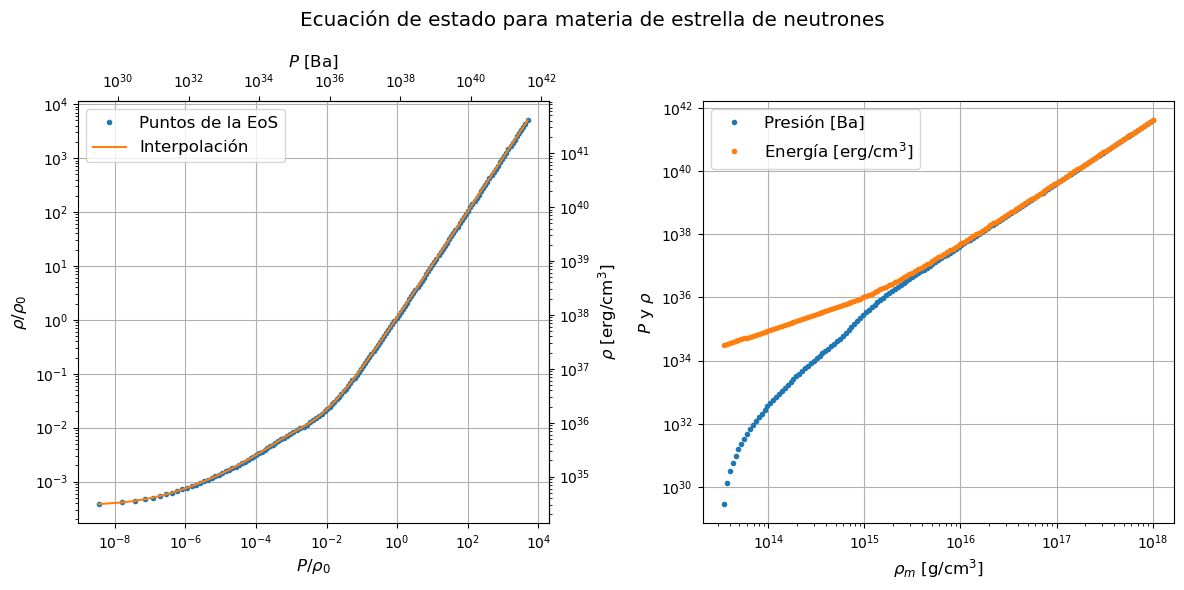
\includegraphics[width=0.95\linewidth]{Figuras/materia_estelar_base}
	\caption[Ecuación de estado para el núcleo de estrellas de neutrones.]{Ecuación de estado para el núcleo de estrellas de neutrones empleando teoría relativista de campo medio. Se usaron los parámetros $\left(\frac{g_\sigma}{m_\sigma}\right)^2=12.684\,\text{fm}^2$, $\left(\frac{g_\omega}{m_\omega}\right)^2=7.148\,\text{fm}^2$, $\left(\frac{g_\rho}{m_\rho}\right)^2=4.410\,\text{fm}^2$, $b=5.610\times10^{-3}$, $c=-6.986\times10^{-3}$.}
	\label{fig:materiaestelarbase}
\end{figure}


\subsection{Materia en Saturación Nuclear}

Si suprimimos los electrones libres del modelo (\ref{eq:lagrangiano}) y consideramos materia nuclear simétrica ($n_p = n_n$), el sistema se reduce a un fluido de nucleones interactuando mediante los campos mesónicos. Este sistema idealizado permite estudiar las propiedades de la materia nuclear en saturación, que corresponde a la densidad a la cual la materia nuclear alcanza su estado de mínima energía por nucleón. Mediante la materia a densidad de saturación es posible calibrar modelos microscópicos de la ecuación de estado nuclear pues tenemos mayor acceso experimental. Se caracteriza por cinco parámetros empíricos que añaden restricciones obligatorias para cualquier teoría microscópica válida \cite{kumarTheoreticalExperimentalConstraints2024}.

La densidad de saturación nuclear $n_0$ define la densidad a la cual la materia nuclear simétrica alcanza su estado de mínima energía de enlace por nucleón $\frac{B}{A}\big|_0  = \frac{\rho(n_0)}{n_0} - m$. Tras ajustar datos de 1654 núcleos en su estado base con N, Z $\geq 8$ a un modelo semi-empírico no relativista de gota líquida, se obtienen valores de $n_0 = 0.16114\, \text{fm}^{-3}$ y $\tfrac{B}{A}\big|_0 = -16.24\, \text{MeV}$, despreciando el término de superficie y el de Coulomb \cite{kumarTheoreticalExperimentalConstraints2024, myersNuclearPropertiesAccording1996}. En nuestro modelo (\ref{eq:lagrangiano}), estas propiedades de saturación se determinan numéricamente hallando el mínimo de la función $\tfrac{B}{A}(n_B)$ en ausencia de electrones, como se muestra de ejemplo en la figura \ref{fig:saturacionbase}.

\begin{figure}[h]
	\centering
	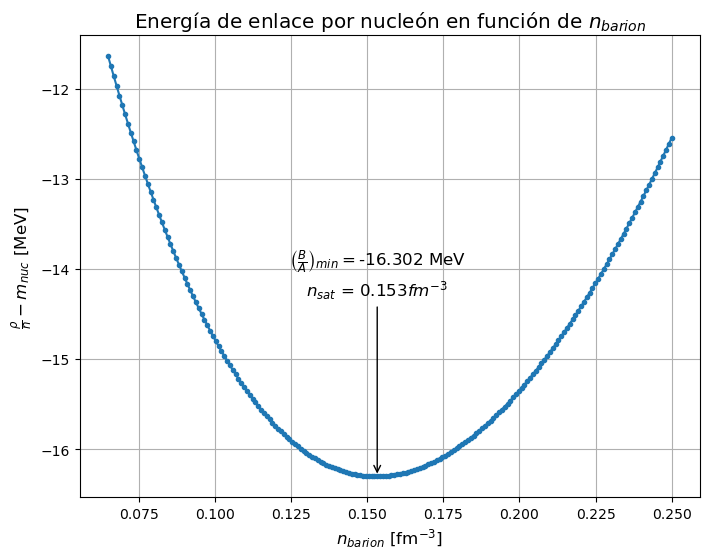
\includegraphics[width=0.7\linewidth]{Figuras/saturacion_base}
	\caption[Energía de enlace por nucleón en saturación nuclear]{Energía de enlace por nucleón en función de la densidad bariónica para materia nuclear simétrica sin electrones. La densidad de saturación $n_0$ y la energía de enlace por nucleón en saturación $\frac{B}{A}\big|_0$ se señalan en el mínimo. Se usaron los parámetros $\left(\frac{g_\sigma}{m_\sigma}\right)^2=12.684\,\text{fm}^2$, $\left(\frac{g_\omega}{m_\omega}\right)^2=7.148\,\text{fm}^2$, $\left(\frac{g_\rho}{m_\rho}\right)^2=4.410\,\text{fm}^2$, $b=5.610\times10^{-3}$, $c=-6.986\times10^{-3}$.}
	\label{fig:saturacionbase}
\end{figure}

El módulo de compresibilidad nuclear $K_0$ caracteriza la rigidez de la materia nuclear ante compresiones alrededor del punto de saturación:

\begin{equation*}
	K_0 = 9n_0^2 \frac{\partial^2}{\partial n^2}\left(\frac{\rho}{n}\right)\bigg|_{n=n_0}.
\end{equation*}

Este parámetro es determinante para la extrapolación de la ecuación de estado a densidades supranucleares, y es estimado mediate las resonancias monopolares en núcleos pesados. Considerando un modelo de cadena de núcleos para esta resonancia en $^{208}$Pb, se obtiene $K_0 = 230 \pm 40$ MeV \cite{kumarTheoreticalExperimentalConstraints2024, khanConstrainingNuclearEquation2012}. Esta cantidad está relacionada algebraicamente con cantidades del modelo con materia simétrica en saturación:

\begin{equation}
	\begin{gathered}
		K_0 = \frac{6}{\pi^2}A_\omega p_F^3 + \frac{3p_F^2}{\sqrt{p_F^2 + (m-x_\sigma)^2}} - \frac{6A_\sigma}{\pi^2}\frac{p_F^3(m-x_\sigma)^2}{p_F^2+(m-x_\sigma)^2}F^{-1}, \\
		F = 1 + A_\sigma x_\sigma[2bm+3cx_\sigma]+\frac{2A_\sigma}{\pi^2}\int_0^{p_F} \frac{p^4 dp}{(p^2+(m-x_\sigma)^2)^{3/2}},
	\end{gathered}
	\label{eq:modulo_compresibilidad}
\end{equation}

donde $A_i = (g_i/m_i)^2$ y $x_\sigma = g_\sigma \sigma$. 

La energía de simetría $a_\text{sym}$ cuantifica el costo energético de desviarse de la composición simétrica. Se define como:

\begin{equation*}
	a_\text{sym} = \frac{1}{2} \frac{\partial^2}{\partial t^2}\left(\frac{E}{A}\right)\bigg|_{t=0},
\end{equation*}

donde $t = (n_n - n_p)/n_B$ es el parámetro de asimetría de isospín. La pendiente de la energía de simetría $L_0$ describe la dependencia con la densidad de la energía de simetría alrededor de la densidad de saturación:

\begin{equation*}
	L_0 = 3n_0 \frac{\partial a_\text{sym}}{\partial n}\bigg|_{n=n_0},
\end{equation*}

y estas dos cantidades, tras una revisión de 28 estimaciones de experimentos tanto terrestres como de observaciones astronómicas de estrellas de neutrones, se estiman valores representativos de $a_\text{sym} = 31.6 \pm 2.7$ MeV y $L_0 = 58.9 \pm 16$ MeV \cite{kumarTheoreticalExperimentalConstraints2024, liUnderstandingAstrophysicalEffects2019}. Es de notar que, si bien el valor fiducial tiene una baja incertidumbre, las estimaciones individuales de $L_0$ varían ampliamente, con intervalos de confianza que oscilan entre 20 y 120 MeV debido a la dificultad para acceder a materia altamente asimétrica en el laboratorio. En nuestro modelo, estas cantidades pueden calcularse como:
\vspace{-6pt}
\begin{align}
	a_\text{sym} &= \frac{p_F^2}{6\sqrt{p_F^2 + (m-x_\sigma)^2}} + \frac{1}{8}A_\rho n_B, \label{eq:energia_simetria} \\
	L_0 &= \frac{p_F^2}{3\sqrt{p_F^2 + (m-x_\sigma)^2}}\left(1 - \frac{p_F^2}{p_F^2 + (m-x_\sigma)^2}\right) + \frac{3}{8}A_\rho n_B. \label{eq:pendiente_simetria}
\end{align}

Estas cinco propiedades empíricas ($n_0$, $\frac{B}{A}\big|_0$, $K_0$, $a_\text{sym}$, $L_0$) definen restricciones que cualquier ecuación de estado microscópica debe satisfacer para ser físicamente viable. En el contexto de la teoría relativista de campo medio, estas propiedades y sus incertidumbres se utilizan para determinar el espacio de parámetros del modelo físicamente aceptable.

\subsection{Corteza de la estrella}

El modelo de teoría relativista de campo medio desarrollado es una descripción de la materia nuclear en el régimen de alta densidad, específicamente para densidades bariónicas superiores a aproximadamente $0.1$ fm$^{-3}$ o $\rho_m \gtrsim 1.7 \times 10^{14}$ g/cm$^3$, donde las interacciones nucleón-nucleón dominan la dinámica del sistema y la aproximación de campo medio tiene sentido. Sin embargo, las estrellas de neutrones presentan una estructura estratificada que incluye regiones de menor densidad donde esta aproximación deja de ser aplicable. La corteza de la estrella, que se extiende desde la superficie hasta el núcleo denso, abarca un rango de densidades de varios órdenes de magnitud y requiere tratamientos teóricos distintos según el régimen de densidad considerado \cite{shapiroBlackHolesWhite2008}.

Para densidades inferiores al punto de goteo de neutrones ($n_{\text{drip}} \approx 2.4\times10^{-4}$ fm$^{-3}$ o $\rho \approx 4 \times 10^{11}$ g/cm$^3$), la materia se compone de una red cristalina de núcleos pesados embebidos en un gas degenerado de electrones, configuración conocida como corteza externa. En este régimen, la ecuación de estado BPS (Baym, Pethick y Sutherland, 1971) \cite{baymGroundStateMatter1971} describe consistentemente con base en la minimización de la energía del estado base de núcleos atómicos para cada densidad, junto con la contribución del gas de electrones relativista. El modelo BPS determina la composición nuclear óptima mediante la competencia entre la energía de masa nuclear, la energía de Coulomb de la red, y la presión del gas electrónico. Por encima de la densidad de goteo de neutrones y hasta densidades del orden de $0.2$ fm$^{-3}$ o $\rho \approx 3.2 \times 10^{14}$ g/cm$^3$ se encuentra la corteza interna, donde los núcleos coexisten con un gas de neutrones libres además del gas de electrones. En este régimen, la ecuación de estado BBP (Baym, Bethe y Pethick, 1971) \cite{baymNeutronStarMatter1971} describe la materia mediante un modelo de gota líquida que considera las contribuciones energéticas de los núcleos, el gas de neutrones libres, y las interacciones nucleares efectivas de la red. Este modelo determina autoconsistentemente la composición nuclear y la fracción de neutrones libres mediante la minimización de la energía total del sistema, que incluye términos de energía de superficie, energía de Coulomb, y energía de simetría nuclear.

El alcance del presente estudio se concentra en la descripción microscópica de la materia nuclear en el régimen de altas energías en las estrellas de neutrones, donde las densidades superan varias veces la densidad de saturación $n_0$, justificando el uso de la teoría relativista de campo medio. Por esta razón, utilizamos las ecuaciones de estado estándar BPS y BBP como entrada externa para integrar las ecuaciones de estructura en las regiones de baja densidad, sin profundizar en los detalles microscópicos de su construcción fuera del marco de este trabajo.

Para construir una ecuación de estado unificada que abarque todo el rango de densidades presente en la estrella, desde la superficie hasta el núcleo, empleamos el método de interpolación \href{https://es.wikipedia.org/wiki/Interpolador_c\%C3\%BAbico_de_Hermite}{PCHIP} (Piecewise Cubic Hermite Interpolating Polynomial), que garantiza una transición suave y monótona entre las diferentes ecuaciones de estado. Este método de interpolación preserva la forma de los datos y evita oscilaciones no físicas que podrían introducir otros métodos de interpolación polinómica. Definimos la densidad de empalme entre la ecuación de estado BBP y nuestro modelo de teoría relativista de campo medio en $n_B = 0.062$ fm$^{-3}$, correspondiente a una densidad de masa de aproximadamente $1.04 \times 10^{14}$ g/cm$^3$. Esta elección se fundamenta en la necesidad de garantizar la causalidad del fluido en toda la estrella, es decir, que la velocidad del sonido $c^2_s = dP/d\rho$ no exceda la velocidad de la luz $c$ en ningún punto. El resultado de esta interpolación para un conjunto de parámetros de ejemplo y su comprobación de causalidad se muestra en la figura \ref{fig:causalidadmateriabase}

\begin{figure}[h]
	\centering
	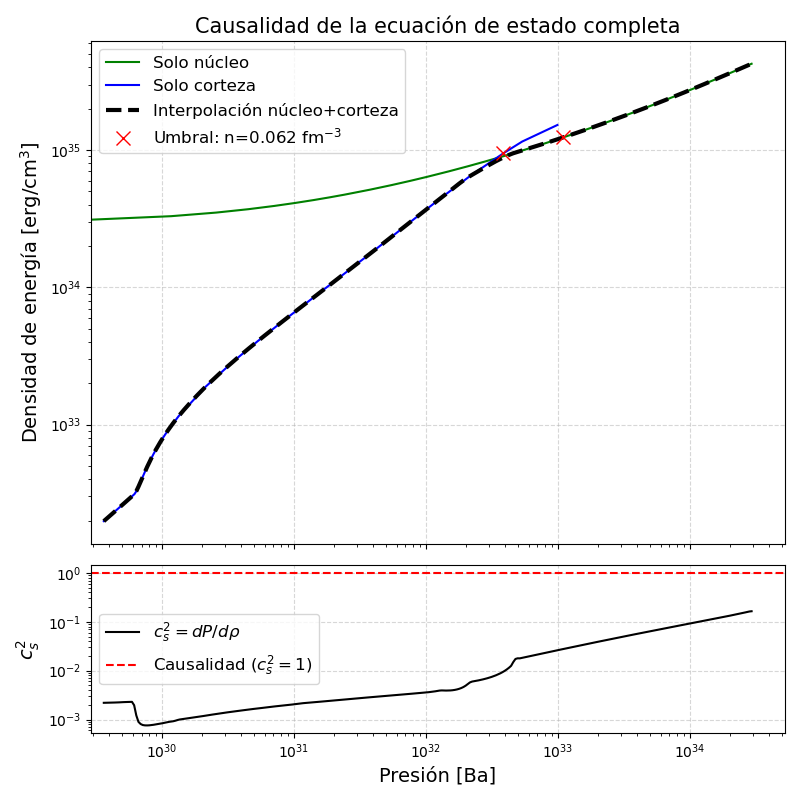
\includegraphics[width=0.7\linewidth]{Figuras/causalidad_materia_estelar_completa}
	\caption[Ecuación de estado unificada y causalidad.]{Ecuación de estado unificada para la estrella de neutrones, construida mediante interpolación PCHIP entre las ecuaciones de estado BPS, BBP y el modelo RMFT. El panel inferior muestra el cuadrado de la velocidad del sonido $c_s^2$ para verificar la condición de causalidad. Se usaron los parámetros $\left(\frac{g_\sigma}{m_\sigma}\right)^2=12.684\,\text{fm}^2$, $\left(\frac{g_\omega}{m_\omega}\right)^2=7.148\,\text{fm}^2$, $\left(\frac{g_\rho}{m_\rho}\right)^2=4.410\,\text{fm}^2$, $b=5.610\times10^{-3}$, $c=-6.986\times10^{-3}$.}
	\label{fig:causalidadmateriabase}
\end{figure}

% Figura: Interpolación PCHIP
% [Espacio para figura mostrando P vs rho para BPS, BBP, interpolación PCHIP, y modelo RMFT, 
% con énfasis en la región de empalme en n_B = 0.062 fm^{-3}. Incluir panel secundario 
% mostrando la velocidad del sonido v_s/c para verificar causalidad (v_s < c) en toda la región.]
